\section{Разработка и описание программных модулей}



\subsection{Jupyter Notebook}

При написании кода приходится при каждом запуске скрипта Python,
снова начитатся обучать нейронная сеть.
Чтобы такого небыло можно поблочно выполнять, перевыполнять Python код в Jupyter Notebook.
Скриншот Jupyter Notebook на
рисунке~\textbf{\ref{fig:4_JupyterNotebook} (стр. \pageref{fig:4_JupyterNotebook})}.

\begin{figure}[!htbp]
    \centering
    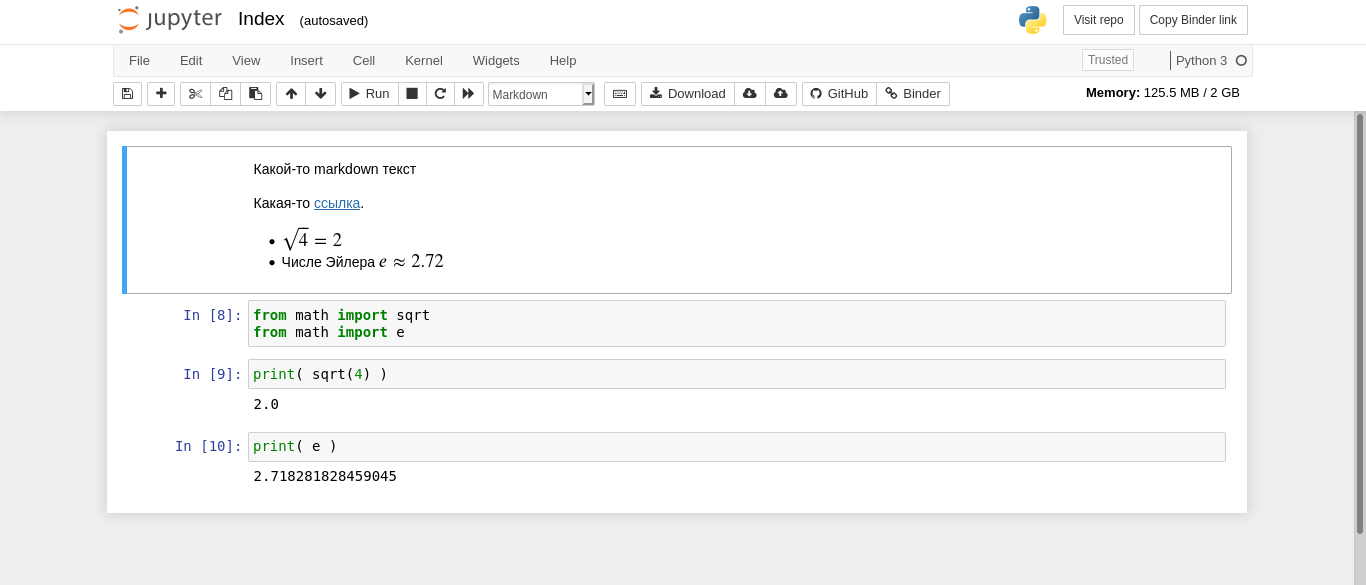
\includegraphics[width=16cm]
    {../_INCLUDES/main/4/JupyterNotebook.png}
    \caption{Jupyter Notebook}
    \label{fig:4_JupyterNotebook}
\end{figure}



\subsection{Google Colaboratory}

Jupyter Notebook - это удобно, но пользуя веб версией мы не получаем все библиотеки Python.
В итоге приходится скачивать Jupyter Notebook на компьютер и ручками скачивать библиотеки,
такие как numpy и tensorflow. Также для обучения нейронной сети на tensorflow нужен графический процессор. Эти две проблемы решает Google Colaboratory, который содержит различные библиотеки Python и дает доступ к другой машине, которая будет обучать нейронную сеть даже с телефона.
Скриншот Google Colaboratory на
рисунке~\textbf{\ref{fig:4_GoogleColaboratory} (стр. \pageref{fig:4_GoogleColaboratory})}.

\begin{figure}[!htbp]
    \centering
    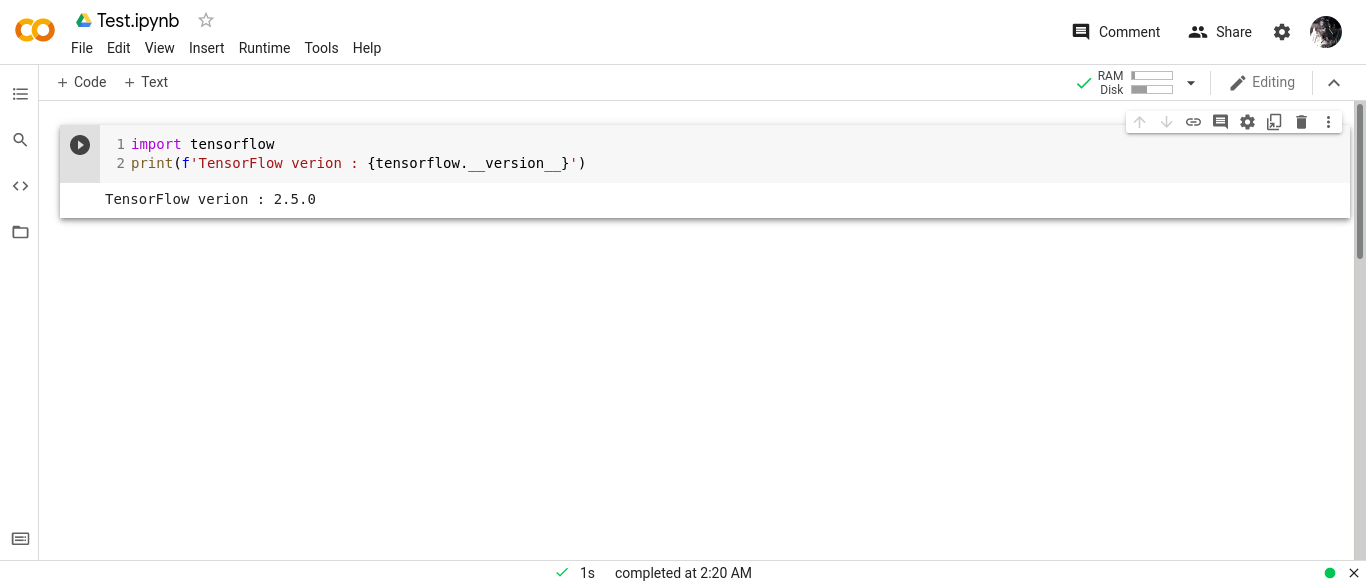
\includegraphics[width=16cm]
    {../_INCLUDES/main/4/GoogleColaboratory.png}
    \caption{Google Colaboratory}
    \label{fig:4_GoogleColaboratory}
\end{figure}



\subsection{Google Colaboratory секции}



\subsubsection*{Секция библиотек}

В секции библиотек подключаем следующие библиотеки:

\begin{enumerate}
    \item numpy - для создания массивов
    \item matplotlib.pyplot - для рисования графиков и картинок
    \item tensorflow - фреймворк
    \item tensorflow.keras - подключение библиотеки keras
    \item tensorflow.keras.layers - для слоёв Flatten и Dense
    \item tensorflow.keras.datasets - для базы данных mnist
\end{enumerate}

\begin{lstlisting}[language=Python,]
    import numpy as np
    import matplotlib.pyplot as plt
    import tensorflow
    from tensorflow.keras.datasets import mnist
    from tensorflow import keras
    from tensorflow.keras.layers import Dense, Flatten
\end{lstlisting}



\subsubsection*{Секция загрузки БД mnist}

\subparagraph{Функция tensorflow.keras.datasets.mnist.load\_data()} \hspace{0pt}

\underline{Входные параметры}: нет.

\underline{Назначение}: загружает в кортедж кортеджей картинки и результат картинок для обучающей и тестовой выборки.

\underline{Возвращаемые данные}: кортедж кортеджей.

\begin{lstlisting}[language=Python,]
    (x_train, y_train), (x_test, y_test) = mnist.load_data()
\end{lstlisting}

Где <<\verb|x_train|>> - изображения цифр обучающей выборки.

Где <<\verb|у_train|>> - вектор соответсвующих значений цифр,
если на i-отом изображении нарисовано 5, то \verb|y_train[i] = 5|.

Где <<\verb|x_test|>> - изображения цифр тестовой выборки.

Где <<\verb|у_test|>> - вектор соответствующих значений цифр для тестовой выборки,
если на i-отом изображении нарисовано 5, то \verb|y_test[i] = 5|.



\subsubsection*{Секция нормирования входных параметров}

В базе данных MNIST изображения рукописных цифр черно-белые. Преобразовав изображения в массив мы имеем градацию цветов в диапазоне от единицы до 255. Максимальное число 255. Если мы разделим каждый пиксель на 255, то получим массив из значение не от 1 до 255, а со значениями от нуля до единицы, которые можем подавать на входные нейроны.

\begin{lstlisting}[language=Python,]
    # стандартизация входных данных
    x_train = x_train / 255
    x_test = x_test / 255
\end{lstlisting}



\newpage



\subsubsection*{Секция классификации выходного слоя}

\subparagraph{Функция tensorflow.keras.datasets.mnist.load\_data()} \hspace{0pt}

\underline{Входные параметры}:

\begin{enumerate}
    \item y - массив чисел
    \item num\_classes - количество классов
\end{enumerate}

\underline{Назначение}: создаст массив размером num\_classes, в который под цифрой запишет 1.

Например, если это число 0, то массив [1,0,0,0,0,0,0,0,0,0].

Например, если это число 1, то массив [0,1,0,0,0,0,0,0,0,0].

Например, если это число 2, то массив [0,0,1,0,0,0,0,0,0,0].

Например, если это число 3, то массив [0,0,0,1,0,0,0,0,0,0].

Например, если это число 4, то массив [0,0,0,0,1,0,0,0,0,0].

Например, если это число 5, то массив [0,0,0,0,0,1,0,0,0,0].

Например, если это число 6, то массив [0,0,0,0,0,0,1,0,0,0].

Например, если это число 7, то массив [0,0,0,0,0,0,0,1,0,0].

Например, если это число 8, то массив [0,0,0,0,0,0,0,0,1,0].

Например, если это число 9, то массив [0,0,0,0,0,0,0,0,0,1].

\underline{Возвращаемые данные}: кортедж кортеджей.

\begin{lstlisting}[language=Python,]
    y_train_cat = keras.utils.to_categorical(y_train, 10)
    y_test_cat = keras.utils.to_categorical(y_test, 10)
\end{lstlisting}



\subsubsection*{Секция моделирования нейронной сети}


\subparagraph{Функция keras.Sequential} \hspace{0pt}

\underline{Входные параметры}: список слоев нейронной сети.

\underline{Назначение}: создает объект модель нейронной сети, у которой появляються методы.

\underline{Возвращаемые данные}: object - объект модели.

\subparagraph{} \hspace{0pt}

Flatten - создает слой, который будет брать значения пикселей картинки построчно.

Dense - создаёт слой, который связывает нейронны предыдущего слоя с текущим.

\begin{lstlisting}[language=Python,]
    model = keras.Sequential([
        Flatten(input_shape=(28, 28, 1)),
        Dense(128, activation='relu'),
        Dense(10, activation='softmax')
    ])
\end{lstlisting}

\subparagraph{Метод .summary} \hspace{0pt}

\underline{Входные параметры}: нет.

\underline{Назначение}: печатает характеристики созданной модели.

\underline{Возвращаемые данные}: None.


\begin{lstlisting}[language=Python,]
    print( model.summary() )
\end{lstlisting}



\subsubsection*{Секция компиляции нейронной сети}

\subparagraph{Метод .compile} \hspace{0pt}

\underline{Входные параметры}:
\begin{enumerate}
    \item (необязательный) optimizer - тип оптимизации;
    \item (необязательный) loss - функция потерь;
    \item (необязательный) metrics - метрика.
\end{enumerate}

\underline{Назначение}: компилирует нейронную сеть.

\underline{Возвращаемые данные}: None.

\begin{lstlisting}[language=Python,]
    model.compile(
        optimizer='adam',
        loss='categorical_crossentropy',
        metrics=['accuracy']
    )
\end{lstlisting}



\newpage



\subsubsection*{Секция обучения нейронной сети}


\subparagraph{Метод .fit} \hspace{0pt}

\underline{Входные параметры}:
\begin{enumerate}
    \item x\_train - входное обучающее множество;
    \item y\_train\_cat - требуемые значения на выходе;
    \item (необязательный) batch\_size - размер batch'a (после скольки изображений будет меняться веса);
    \item (необязательный) epochs - количество эпох;
    \item (необязательный) validation\_split - разбиение обучающей выборки.
\end{enumerate}

\underline{Назначение}: выводит информацию при обучении на каждой эпохе.

\underline{Возвращаемые данные}: object.

\begin{lstlisting}[language=Python,]
    model.fit(
        x_train,
        y_train_cat,
        batch_size=32,
        epochs=5,
        validation_split=0.2
    )
\end{lstlisting}



\subsubsection*{Секция оценки качества нейронной сети на тестовой выборке}

\subparagraph{Метод .evaluate} \hspace{0pt}

\underline{Входные параметры}:
\begin{enumerate}
    \item x\_test - картинки тестовой выборки;
    \item y\_test\_cat - ожидаемый результат тестовой выборки.
\end{enumerate}

\underline{Назначение}: выводит в списке значение потерь и значение показатель обучения.

\underline{Возвращаемые данные}: list - список.

\begin{lstlisting}[language=Python,]
    model.evaluate(x_test, y_test_cat)
\end{lstlisting}

\begin{lstlisting}[name=Вывод в консоль,]
    [0.12078429013490677, 0.9781000018119812]
\end{lstlisting}



\subsubsection*{Секция вывода пердсказанного числа и картинки}

\subparagraph{Функция print\_info\_about\_image\_by\_index(n)} \hspace{0pt}

\underline{Входные параметры}: n - индекс картинки.

\underline{Назначение}: выводит картинку, а в заголовке предсказанное значение.

\underline{Возвращаемые данные}: нет.

\begin{lstlisting}[language=Python,]
    def print_info_about_image_by_index(n):
        x = np.expand_dims( x_test[n], axis=0 )
        res = model.predict(x)
        print(f'Десять выходных значений: {res}')
        print(f'Распознанная цифра : {np.argmax(res)}')
        print()
        plt.imshow(x_test[n], cmap=plt.cm.binary)
        plt.show()
\end{lstlisting}

\begin{lstlisting}[language=Python,]
    # 10 раз вызвали функцию
    for i in range(0, 10):
        print_info_about_image_by_index(i)
\end{lstlisting}

Результат на
рисунке~\textbf{\ref{fig:4_img_and_result} (стр. \pageref{fig:4_img_and_result})}.

\begin{figure}[!htp]
    \centering

    \begin{minipage}[h]{0.19\linewidth}
        \centering
        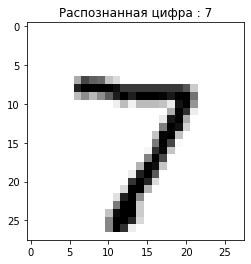
\includegraphics[width=\linewidth]
        {../_INCLUDES/main/4/result1.png}
    \end{minipage}
    \hfill
    \begin{minipage}[h]{0.19\linewidth}
        \centering
        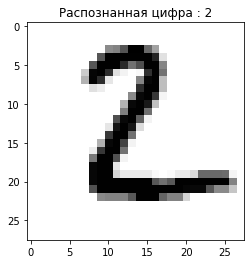
\includegraphics[width=\linewidth]
        {../_INCLUDES/main/4/result2.png}
    \end{minipage}
    \hfill
    \begin{minipage}[h]{0.19\linewidth}
        \centering
        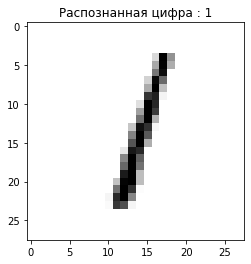
\includegraphics[width=\linewidth]
        {../_INCLUDES/main/4/result3.png}
    \end{minipage}
    \hfill
    \begin{minipage}[h]{0.19\linewidth}
        \centering
        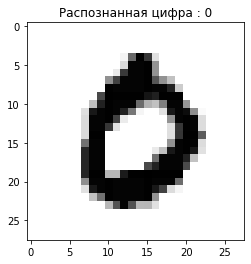
\includegraphics[width=\linewidth]
        {../_INCLUDES/main/4/result4.png}
    \end{minipage}
    \hfill
    \begin{minipage}[h]{0.19\linewidth}
        \centering
        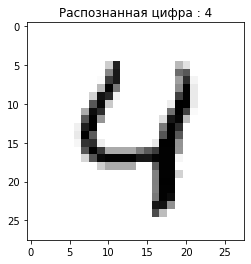
\includegraphics[width=\linewidth]
        {../_INCLUDES/main/4/result5.png}
    \end{minipage}


    \begin{minipage}[h]{0.19\linewidth}
        \centering
        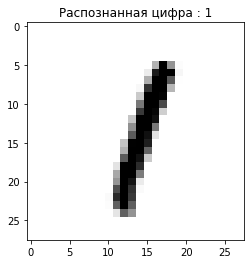
\includegraphics[width=\linewidth]
        {../_INCLUDES/main/4/result6.png}
    \end{minipage}
    \hfill
    \begin{minipage}[h]{0.19\linewidth}
        \centering
        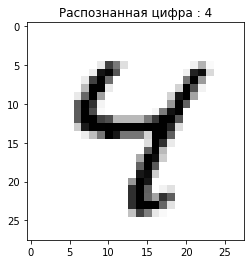
\includegraphics[width=\linewidth]
        {../_INCLUDES/main/4/result7.png}
    \end{minipage}
    \hfill
    \begin{minipage}[h]{0.19\linewidth}
        \centering
        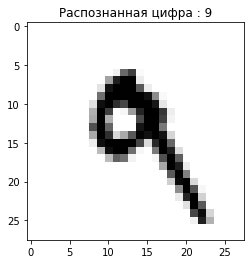
\includegraphics[width=\linewidth]
        {../_INCLUDES/main/4/result8.png}
    \end{minipage}
    \hfill
    \begin{minipage}[h]{0.19\linewidth}
        \centering
        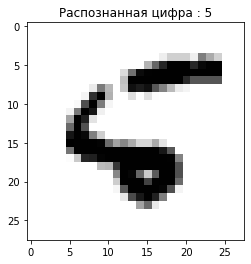
\includegraphics[width=\linewidth]
        {../_INCLUDES/main/4/result9.png}
    \end{minipage}
    \hfill
    \begin{minipage}[h]{0.19\linewidth}
        \centering
        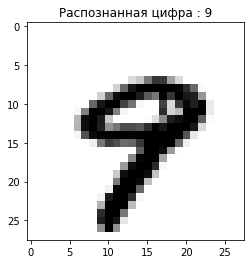
\includegraphics[width=\linewidth]
        {../_INCLUDES/main/4/result10.png}
    \end{minipage}

    \caption{Картинка и результат нейронной сети}
    \label{fig:4_img_and_result}
\end{figure}



\subsubsection*{Отбор не правильных ответов}

При тестировании у нас есть уже какие-то ответы нейронной сети. То что изображено на картинке мы также знаем. Если то, что изображено на картинке совпадает с результатом выданным нейронной сетью, то добавляем в массив True, иначе False. Неправльно распознанные изображения у нас с меткой False. С помощью маски мы отбираем неправильные изображения.

\begin{lstlisting}[language=Python,]
    mask = pred == y_test
    x_false = x_test[~mask]
    p_false = pred[~mask]
    print(f'Размерность x_false : {x_false.shape}')
    print(f'Размерность p_false : {p_false.shape}')
\end{lstlisting}

\begin{lstlisting}[name=Вывод в консоль,]
    Размерность x_false : (243, 28, 28)
    Размерность p_false : (243,)
\end{lstlisting}

В итоге сеть не распознала 243 изображения.



\subsubsection*{Вывод не правильных картинок}

\begin{lstlisting}[language=Python,]
    # Вывод первых 243 неверных результатов
    plt.figure(figsize=(10,10)) # размер в дюймах
    for i in range(243):
        plt.subplot(13,20,i+1)  # расположить картинки в 13x20
        plt.xticks([])          # не выводить оси по x
        plt.yticks([])          # не выводить оси по y
        plt.title(p_false[i])   # печать в заголовок картинки цифру
        plt.imshow(x_false[i], cmap=plt.cm.binary) # печатает в рамку
    plt.show()                  # напечатать картинку
\end{lstlisting}

Не правильно распознанные картинки изображены на
рисунке~\textbf{\ref{fig:4_not_right_imgs} (стр. \pageref{fig:4_not_right_imgs})}.

\begin{figure}[!htbp]
    \centering
    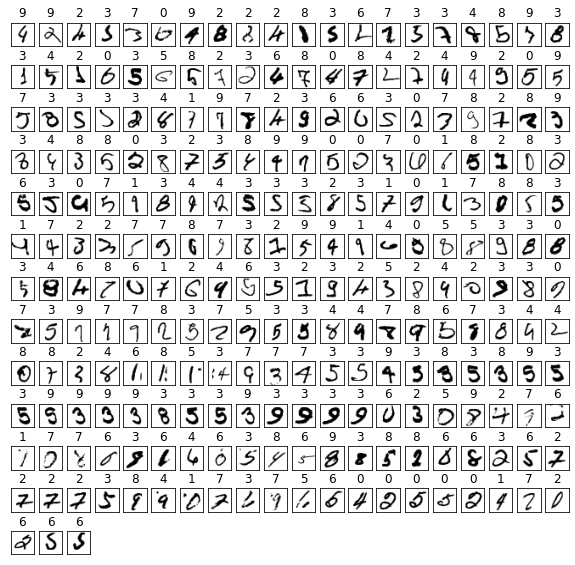
\includegraphics[width=16cm]
    {../_INCLUDES/main/4/not_right_imgs.png}
    \caption{Не правльно распознанные цифры}
    \label{fig:4_not_right_imgs}
\end{figure}